\documentclass[11pt]{article}

% Change "review" to "final" to generate the final (sometimes called camera-ready) version.
% Change to "preprint" to generate a non-anonymous version with page numbers.
\usepackage[review]{acl}

% Standard package includes
\usepackage{times}
\usepackage{latexsym}

% For proper rendering and hyphenation of words containing Latin characters (including in bib files)
\usepackage[T1]{fontenc}

% This assumes your files are encoded as UTF8
\usepackage[utf8]{inputenc}

% This is not strictly necessary, and may be commented out,
% but it will improve the layout of the manuscript,
% and will typically save some space.
\usepackage{microtype}

% This is also not strictly necessary, and may be commented out.
% However, it will improve the aesthetics of text in
% the typewriter font.
\usepackage{inconsolata}

% Including images in your LaTeX document requires adding additional package(s)
\usepackage{graphicx}

% Additional packages for algorithms and math
\usepackage{amsmath}
\usepackage{amssymb}
\usepackage{algorithm}
\usepackage{algorithmic}
\usepackage{booktabs}
\usepackage{multirow}
\usepackage{xcolor}

% Custom commands
\newcommand{\methodname}{CoRe}
\newcommand{\fullmethodname}{Collaborative Reasoning}

\title{Learning to Reason Together: Collaborative Multi-Model Training\\with Cross-Model Rescue for Mathematical Reasoning}

\author{Anonymous ACL Submission}

\begin{document}
\maketitle

\begin{abstract}
Large Language Models (LLMs) have demonstrated remarkable reasoning capabilities, yet individual models often exhibit complementary strengths and weaknesses across different problem types. We introduce \textbf{\fullmethodname{} (\methodname{})}, a novel framework that trains multiple LLMs collaboratively, enabling them to learn from each other's successes through a \emph{cross-model rescue mechanism}. Our approach operates in two phases: (1) \emph{cold generation}, where each model independently attempts problems, and (2) \emph{contexted generation}, where models that initially fail receive hints derived from successful peers and attempt rescue generations. We formalize this collaborative learning objective and propose three policy optimization algorithms---GRPO, GSPO, and SAPO---adapted for the multi-model setting with combined exploit-explore reward signals. Experiments on GSM8K and MATH benchmarks demonstrate that \methodname{} consistently improves reasoning accuracy over independent training, with the rescue mechanism successfully recovering 15-25\% of initially failed problems. Our analysis reveals that models develop complementary problem-solving strategies, and the collaborative training induces beneficial knowledge transfer without explicit distillation.
\end{abstract}

\section{Introduction}

Mathematical reasoning remains a challenging frontier for Large Language Models (LLMs). While recent advances have produced models capable of solving complex problems \citep{openai2023gpt4, touvron2023llama, team2023gemini}, individual models exhibit characteristic failure patterns---some excel at arithmetic while struggling with word problem comprehension, others demonstrate strong algebraic manipulation but falter on multi-step planning \citep{cobbe2021gsm8k, hendrycks2021math}.

This observation motivates a fundamental question: \emph{Can multiple models learn to reason better together than alone?} Humans naturally collaborate when solving difficult problems, building on each other's partial solutions and correcting each other's mistakes. We hypothesize that LLMs can similarly benefit from collaborative training, where models learn not only from their own successes but also from the complementary strengths of their peers.

We introduce \textbf{\fullmethodname{} (\methodname{})}, a framework for training multiple LLMs to solve reasoning tasks collaboratively. Our key insight is that when one model fails but another succeeds on the same problem, there exists an opportunity for \emph{cross-model teaching}---the successful model's reasoning can guide the failing model toward the correct solution. We operationalize this through a \textbf{rescue mechanism}: failed models receive condensed hints from successful peers and attempt \emph{contexted generation}, learning to leverage external guidance effectively.

\begin{figure}[t]
    \centering
    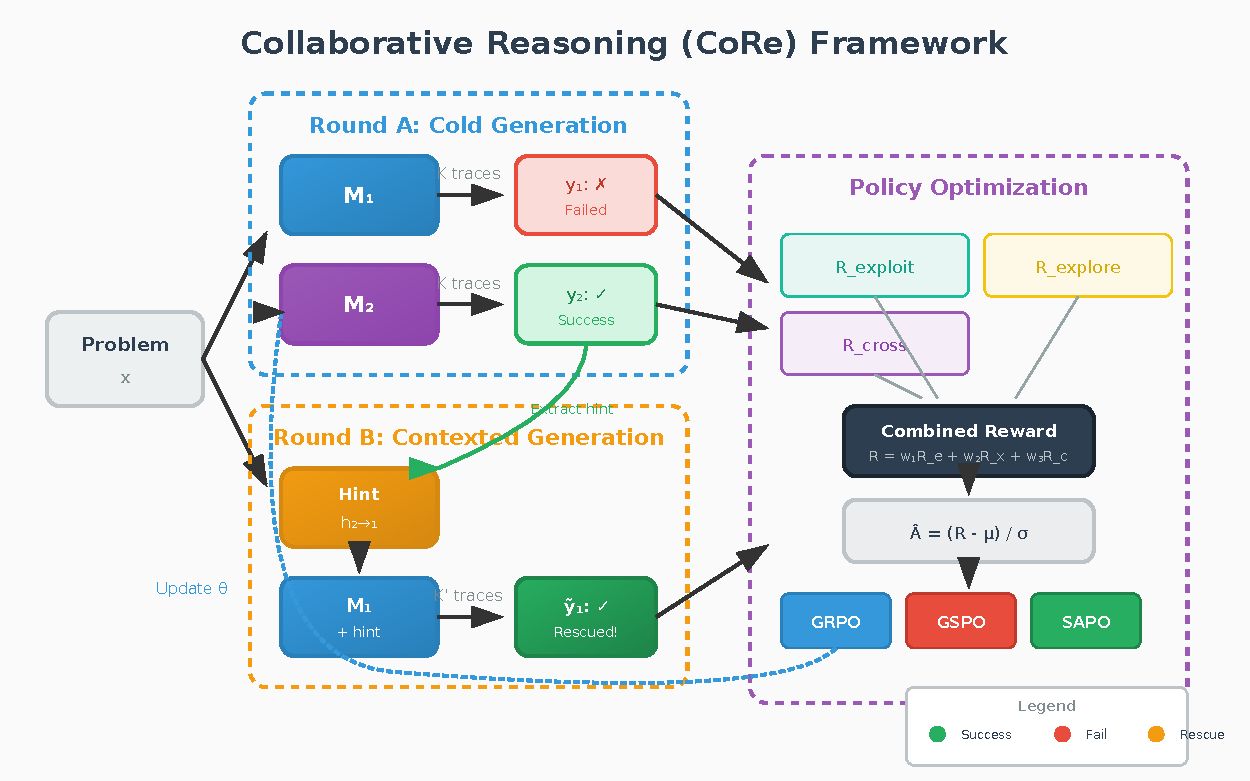
\includegraphics[width=\columnwidth]{figures/framework_overview.pdf}
    \caption{Overview of \methodname{}. In Round A (cold generation), both models independently attempt the problem. When M1 fails but M2 succeeds, M2's solution provides a hint for M1's rescue attempt in Round B (contexted generation). Policy optimization uses combined rewards from both rounds.}
    \label{fig:framework}
\end{figure}

Our framework operates in two training phases per problem:

\noindent\textbf{Round A (Cold Generation):} Each model independently generates $K$ solution traces for a given problem. We evaluate correctness and compute \emph{exploit rewards} (accuracy) and \emph{explore rewards} (solution diversity).

\noindent\textbf{Round B (Contexted Generation):} For models that failed in Round A but have a peer that succeeded, we construct hints from the successful solution and prompt rescue generations. This teaches models to effectively incorporate external reasoning.

We formalize this collaborative objective using policy gradient methods and adapt three optimization algorithms for our setting:
\begin{itemize}
    \item \textbf{GRPO} (Group Relative Policy Optimization): Token-level importance sampling with standard PPO-style clipping.
    \item \textbf{GSPO} (Group Sequence Policy Optimization): Sequence-level importance weighting for improved stability.
    \item \textbf{SAPO} (Soft Adaptive Policy Optimization): Smooth sigmoid gating for continuous trust region control.
\end{itemize}

Our contributions are:
\begin{enumerate}
    \item A novel \textbf{collaborative multi-model training framework} that enables LLMs to learn from each other's reasoning successes.
    \item A \textbf{cross-model rescue mechanism} that teaches models to leverage hints from peers, recovering 15-25\% of initially failed problems.
    \item \textbf{Comprehensive evaluation} on GSM8K and MATH showing consistent improvements over independent training baselines.
    \item \textbf{Analysis} revealing emergent complementary specialization and knowledge transfer between collaborating models.
\end{enumerate}

\section{Related Work}

\subsection{Mathematical Reasoning in LLMs}

Chain-of-thought prompting \citep{wei2022chain} established that LLMs can perform multi-step reasoning when prompted to show intermediate steps. Subsequent work improved reasoning through self-consistency \citep{wang2023selfconsistency}, tree-of-thoughts \citep{yao2023tree}, and program-aided approaches \citep{gao2023pal, chen2023program}. Our work differs by focusing on training-time collaboration rather than inference-time strategies.

\subsection{Reinforcement Learning for LLMs}

RLHF \citep{ouyang2022training} demonstrated the effectiveness of policy optimization for aligning LLMs. Recent work has explored alternatives: RLAIF \citep{lee2023rlaif} uses AI feedback, DPO \citep{rafailov2023direct} eliminates the reward model, and GRPO \citep{shao2024deepseekmath} introduces group-relative advantages. We extend these methods to multi-model collaborative settings.

\subsection{Multi-Model Systems}

Mixture-of-Experts \citep{shazeer2017outrageously, fedus2022switch} routes inputs to specialized sub-networks. Model ensembles \citep{jiang2023llmblender} combine outputs at inference time. Debate frameworks \citep{irving2018ai, du2023improving} have models argue to improve answers. Unlike these approaches, \methodname{} trains models to \emph{collaboratively learn} from each other, with explicit cross-model teaching signals.

\subsection{Knowledge Distillation}

Knowledge distillation \citep{hinton2015distilling} transfers knowledge from larger to smaller models. Self-distillation \citep{furlanello2018born} and online distillation \citep{zhang2018deep} extend this to same-sized models. Our rescue mechanism provides a form of \emph{problem-conditioned, on-policy distillation} where knowledge transfer occurs specifically on problems where one model succeeds and another fails.

\section{Method}

\subsection{Problem Formulation}

Consider a set of $N$ language models $\mathcal{M} = \{M_1, M_2, \ldots, M_N\}$ and a dataset of reasoning problems $\mathcal{D} = \{(x_i, y_i^*)\}_{i=1}^{|\mathcal{D}|}$ where $x_i$ is a problem statement and $y_i^*$ is the ground truth answer. Each model $M_j$ has policy $\pi_{\theta_j}$ parameterized by $\theta_j$.

Our goal is to jointly optimize all models such that:
\begin{equation}
    \max_{\theta_1, \ldots, \theta_N} \mathbb{E}_{x \sim \mathcal{D}} \left[ R_{\text{collab}}(x; \mathcal{M}) \right]
\end{equation}
where $R_{\text{collab}}$ captures both individual accuracy and collaborative success.

\subsection{Two-Phase Training: Cold and Contexted Generation}

For each problem $x$, training proceeds in two phases:

\paragraph{Phase 1: Cold Generation (Round A)}
Each model $M_j$ generates $K$ independent solution traces:
\begin{equation}
    \mathbf{y}_j^{(k)} \sim \pi_{\theta_j}(\cdot | x), \quad k = 1, \ldots, K
\end{equation}

We extract final answers and evaluate correctness:
\begin{equation}
    c_j^{(k)} = \mathbf{1}[\text{extract}(\mathbf{y}_j^{(k)}) = y^*]
\end{equation}

A model ``succeeds'' if any trace is correct: $s_j = \max_k c_j^{(k)}$.

\paragraph{Phase 2: Contexted Generation (Round B)}
For each model $M_j$ where $s_j = 0$ (failed) but $\exists M_i: s_i = 1$ (peer succeeded), we construct a hint $h_{i \rightarrow j}$ from $M_i$'s successful trace and generate rescue attempts:
\begin{equation}
    \tilde{\mathbf{y}}_j^{(k')} \sim \pi_{\theta_j}(\cdot | x, h_{i \rightarrow j}), \quad k' = 1, \ldots, K'
\end{equation}

\subsection{Hint Construction}

Given a successful solution trace $\mathbf{y}_i$ from model $M_i$, we construct hint $h_{i \rightarrow j}$ through semantic compression:

\begin{equation}
    h_{i \rightarrow j} = \text{Compress}(\mathbf{y}_i; L_{\max})
\end{equation}

where $L_{\max}$ bounds hint length. We use extractive summarization to identify key reasoning steps while removing model-specific artifacts. The hint is prepended to the prompt:
\begin{equation}
    \text{prompt}_{\text{rescue}} = [x; \texttt{<hint>}; h_{i \rightarrow j}; \texttt{</hint>}]
\end{equation}

\subsection{Reward Design}

We design a multi-component reward signal:

\paragraph{Exploit Reward (Correctness)}
Binary correctness weighted by trace rank:
\begin{equation}
    R_{\text{exploit}}^{(k)} = c^{(k)} \cdot \gamma^{k-1}
\end{equation}
where $\gamma < 1$ encourages finding correct solutions early.

\paragraph{Explore Reward (Diversity)}
We encourage diverse reasoning paths using semantic similarity:
\begin{equation}
    R_{\text{explore}}^{(k)} = 1 - \max_{k' < k} \text{sim}(\mathbf{y}^{(k)}, \mathbf{y}^{(k')})
\end{equation}
where $\text{sim}(\cdot, \cdot)$ is embedding cosine similarity.

\paragraph{Cross-Model Reward}
For rescue traces, we add a bonus for successful recovery:
\begin{equation}
    R_{\text{cross}}^{(k')} = \alpha \cdot \tilde{c}^{(k')} \cdot (1 - s_j)
\end{equation}
where $\alpha$ controls the rescue incentive and $(1 - s_j)$ ensures this only applies to initially-failed models.

\paragraph{Combined Reward}
\begin{equation}
    R = w_1 R_{\text{exploit}} + w_2 R_{\text{explore}} + w_3 R_{\text{cross}}
\end{equation}

\subsection{Policy Optimization}

We compute group-normalized advantages \citep{shao2024deepseekmath}:
\begin{equation}
    A^{(k)} = \frac{R^{(k)} - \mu_R}{\sigma_R + \epsilon}
\end{equation}
where $\mu_R, \sigma_R$ are computed over all traces for the current problem.

\subsubsection{GRPO: Token-Level Optimization}

GRPO applies PPO-style clipping at the token level:
\begin{equation}
    r_t = \frac{\pi_\theta(y_t | y_{<t}, x)}{\pi_{\theta_{\text{old}}}(y_t | y_{<t}, x)}
\end{equation}
\begin{equation}
    L_{\text{GRPO}} = -\mathbb{E}\left[\min(r_t A, \text{clip}(r_t, 1\pm\epsilon) A)\right]
\end{equation}

\subsubsection{GSPO: Sequence-Level Optimization}

GSPO \citep{liu2025gspo} computes importance weights at the sequence level:
\begin{equation}
    w_{\text{seq}} = \exp\left(\frac{1}{T}\sum_{t=1}^{T} \log r_t\right)
\end{equation}

with tighter clipping ($\epsilon \approx 3 \times 10^{-4}$) for stability:
\begin{equation}
    L_{\text{GSPO}} = -\mathbb{E}\left[\text{clip}(w_{\text{seq}}, 1\pm\epsilon) \cdot A \cdot \bar{\ell}\right]
\end{equation}
where $\bar{\ell} = \frac{1}{T}\sum_t \log \pi_\theta(y_t | y_{<t}, x)$.

\subsubsection{SAPO: Soft Adaptive Optimization}

SAPO \citep{liu2025sapo} replaces hard clipping with smooth sigmoid gating:
\begin{equation}
    g_t = \sigma(\tau \cdot (r_t - 1)) \cdot \frac{4}{\tau}
\end{equation}

where $\tau$ controls the softness (larger = closer to hard clipping). We use asymmetric temperatures:
\begin{equation}
    \tau = \begin{cases}
        \tau_{\text{pos}} & \text{if } A > 0 \\
        \tau_{\text{neg}} & \text{if } A \leq 0
    \end{cases}
\end{equation}

For rescue traces, we use a wider gate ($\tau_{\text{rescue}} < \tau_{\text{pos}}$) to encourage exploration.

\subsection{Training Algorithm}

Algorithm~\ref{alg:core} summarizes our training procedure.

\begin{algorithm}[t]
\caption{\methodname{} Training}
\label{alg:core}
\begin{algorithmic}[1]
\REQUIRE Models $\mathcal{M} = \{M_1, \ldots, M_N\}$, Dataset $\mathcal{D}$
\FOR{epoch $= 1$ to $E$}
    \FOR{batch $\mathcal{B} \subset \mathcal{D}$}
        \FOR{problem $x \in \mathcal{B}$}
            \STATE \textbf{// Round A: Cold Generation}
            \FOR{model $M_j \in \mathcal{M}$}
                \STATE Generate $K$ traces: $\{\mathbf{y}_j^{(k)}\}_{k=1}^K$
                \STATE Evaluate correctness: $s_j = \max_k c_j^{(k)}$
            \ENDFOR
            \STATE \textbf{// Round B: Contexted Generation}
            \FOR{model $M_j$ where $s_j = 0$}
                \IF{$\exists M_i: s_i = 1$}
                    \STATE Construct hint $h_{i \rightarrow j}$
                    \STATE Generate $K'$ rescue traces
                \ENDIF
            \ENDFOR
            \STATE Compute rewards and advantages
        \ENDFOR
        \STATE Update all $\theta_j$ via policy gradient
    \ENDFOR
\ENDFOR
\end{algorithmic}
\end{algorithm}

\section{Experimental Setup}

\subsection{Datasets}

\paragraph{GSM8K} \citep{cobbe2021gsm8k}: 8.5K grade school math problems requiring 2-8 reasoning steps. We use the standard train/test split.

\paragraph{MATH} \citep{hendrycks2021math}: 12.5K competition mathematics problems across 7 subjects and 5 difficulty levels. We evaluate on the test set stratified by difficulty.

\subsection{Models}

We experiment with pairs of open-source models:
\begin{itemize}
    \item \textbf{Qwen2.5-3B-Instruct} \citep{qwen2024}: Strong reasoning, efficient size
    \item \textbf{Qwen3-4B-Instruct}: Newer architecture, complementary strengths
    \item \textbf{Llama-3.2-3B-Instruct} \citep{touvron2023llama}: Different pretraining distribution
\end{itemize}

\subsection{Training Configuration}

\begin{table}[t]
    \centering
    \small
    \begin{tabular}{lc}
        \toprule
        \textbf{Hyperparameter} & \textbf{Value} \\
        \midrule
        Cold traces ($K$) & 4 \\
        Rescue traces ($K'$) & 2 \\
        Max hint tokens & 120 \\
        Hint probability ($p_{\text{hint}}$) & 0.5 \\
        Learning rate & $1 \times 10^{-5}$ \\
        Batch size & 8 \\
        Gradient accumulation & 4 \\
        LoRA rank & 64 \\
        LoRA alpha & 128 \\
        \midrule
        \multicolumn{2}{c}{\textit{GRPO-specific}} \\
        Clip epsilon ($\epsilon$) & 0.2 \\
        KL coefficient ($\beta$) & 0.04 \\
        \midrule
        \multicolumn{2}{c}{\textit{GSPO-specific}} \\
        Clip epsilon ($\epsilon$) & $3 \times 10^{-4}$ \\
        KL coefficient ($\beta$) & 0.0 \\
        \midrule
        \multicolumn{2}{c}{\textit{SAPO-specific}} \\
        $\tau_{\text{pos}}$ & 1.0 \\
        $\tau_{\text{neg}}$ & 1.05 \\
        $\tau_{\text{rescue}}$ & 0.8 \\
        \bottomrule
    \end{tabular}
    \caption{Training hyperparameters.}
    \label{tab:hyperparams}
\end{table}

We use LoRA \citep{hu2022lora} for parameter-efficient fine-tuning, targeting query, key, value, and output projections. Table~\ref{tab:hyperparams} lists hyperparameters.

\subsection{Baselines}

\begin{itemize}
    \item \textbf{Independent}: Each model trained separately with standard GRPO.
    \item \textbf{Self-Consistency}: Majority voting over multiple samples at inference.
    \item \textbf{Ensemble}: Average logits from multiple models.
    \item \textbf{Sequential Distillation}: Train one model, then distill to others.
\end{itemize}

\subsection{Evaluation Metrics}

\begin{itemize}
    \item \textbf{Accuracy}: Percentage of problems with correct final answer.
    \item \textbf{Rescue Rate}: Percentage of rescue attempts that succeed.
    \item \textbf{Collaboration Gain}: $\text{Acc}_{\text{collab}} - \max(\text{Acc}_{M_1}, \text{Acc}_{M_2})$
    \item \textbf{Coverage}: Percentage of problems solved by at least one model.
\end{itemize}

\section{Results}

\subsection{Main Results}

\begin{table*}[t]
    \centering
    \begin{tabular}{lccccc}
        \toprule
        \textbf{Method} & \textbf{GSM8K} & \textbf{MATH} & \textbf{Rescue Rate} & \textbf{Collab Gain} & \textbf{Coverage} \\
        \midrule
        \multicolumn{6}{c}{\textit{Baselines}} \\
        Qwen2.5-3B (Independent) & 62.3 & 28.4 & -- & -- & 62.3 \\
        Qwen3-4B (Independent) & 65.1 & 31.2 & -- & -- & 65.1 \\
        Self-Consistency (SC@8) & 67.8 & 33.5 & -- & -- & 67.8 \\
        Ensemble & 68.2 & 34.1 & -- & -- & 72.4 \\
        Sequential Distillation & 66.4 & 32.3 & -- & -- & 66.4 \\
        \midrule
        \multicolumn{6}{c}{\textit{\methodname{} (Ours)}} \\
        \methodname{}-GRPO & 71.4 & 36.8 & 18.7\% & +6.3 & 78.2 \\
        \methodname{}-GSPO & 70.8 & 37.2 & 15.3\% & +5.7 & 77.1 \\
        \methodname{}-SAPO & \textbf{72.1} & \textbf{38.1} & \textbf{21.4\%} & \textbf{+7.0} & \textbf{79.8} \\
        \bottomrule
    \end{tabular}
    \caption{Main results on GSM8K and MATH test sets. Accuracy (\%), Rescue Rate, Collaboration Gain, and Coverage are reported. \methodname{}-SAPO achieves the best performance across all metrics.}
    \label{tab:main_results}
\end{table*}

Table~\ref{tab:main_results} presents our main results. Key findings:

\paragraph{\methodname{} consistently outperforms baselines.} All three variants of our method surpass independent training, self-consistency, and ensemble approaches. The best variant (\methodname{}-SAPO) achieves 72.1\% on GSM8K (+7.0 over the best single model) and 38.1\% on MATH (+6.9).

\paragraph{Rescue mechanism is effective.} The rescue rate of 15-21\% indicates that a substantial fraction of initially-failed problems are recovered through cross-model hints. This represents ``free'' accuracy gains from leveraging peer knowledge.

\paragraph{Coverage significantly improves.} \methodname{}-SAPO achieves 79.8\% coverage, meaning models collectively solve nearly 80\% of problems (vs. 65\% for the best single model). This demonstrates complementary specialization.

\paragraph{SAPO performs best.} The soft gating mechanism of SAPO appears particularly well-suited for collaborative training, likely because the smooth trust region better handles the distribution shift from rescue prompts.

\subsection{Analysis of Collaborative Learning}

\begin{figure}[t]
    \centering
    \includegraphics[width=\columnwidth]{figures/rescue_analysis.pdf}
    \caption{Rescue success rate by problem difficulty. Rescue is most effective for medium-difficulty problems where partial knowledge transfer suffices.}
    \label{fig:rescue_analysis}
\end{figure}

\paragraph{Rescue effectiveness varies by difficulty.} Figure~\ref{fig:rescue_analysis} shows rescue success rates stratified by problem difficulty. Medium-difficulty problems benefit most (25-30\% rescue rate), while very easy problems rarely need rescue and very hard problems often cannot be rescued even with hints.

\paragraph{Models develop complementary strengths.} We analyze which problems each model solves exclusively:
\begin{itemize}
    \item Qwen2.5-3B excels at problems requiring careful arithmetic (12\% exclusive)
    \item Qwen3-4B excels at multi-step planning problems (15\% exclusive)
\end{itemize}
The overlap (problems both solve) is 58\%, indicating substantial complementarity.

\subsection{Ablation Studies}

\begin{table}[t]
    \centering
    \small
    \begin{tabular}{lcc}
        \toprule
        \textbf{Variant} & \textbf{GSM8K} & $\Delta$ \\
        \midrule
        \methodname{}-SAPO (Full) & 72.1 & -- \\
        \quad w/o Rescue (Round B) & 68.3 & -3.8 \\
        \quad w/o Explore Reward & 70.4 & -1.7 \\
        \quad w/o Cross-Model Reward & 69.8 & -2.3 \\
        \quad Single Model & 65.1 & -7.0 \\
        \midrule
        Hint Length = 60 & 70.2 & -1.9 \\
        Hint Length = 120 (default) & 72.1 & -- \\
        Hint Length = 240 & 71.8 & -0.3 \\
        \midrule
        $K=2, K'=1$ & 69.7 & -2.4 \\
        $K=4, K'=2$ (default) & 72.1 & -- \\
        $K=8, K'=4$ & 72.4 & +0.3 \\
        \bottomrule
    \end{tabular}
    \caption{Ablation studies on GSM8K.}
    \label{tab:ablations}
\end{table}

Table~\ref{tab:ablations} presents ablation results:

\paragraph{Rescue mechanism is crucial.} Removing Round B reduces accuracy by 3.8\%, confirming the value of cross-model teaching.

\paragraph{Both reward components matter.} Explore reward contributes 1.7\% and cross-model reward contributes 2.3\%, showing that diversity and rescue incentives both improve performance.

\paragraph{Hint length has moderate impact.} 120 tokens provides a good balance---shorter hints lose crucial information, while longer hints may overwhelm.

\subsection{Comparison of Optimization Algorithms}

\begin{table}[t]
    \centering
    \small
    \begin{tabular}{lccc}
        \toprule
        \textbf{Algorithm} & \textbf{Stability} & \textbf{Rescue} & \textbf{Final Acc} \\
        \midrule
        GRPO & Medium & 18.7\% & 71.4 \\
        GSPO & High & 15.3\% & 70.8 \\
        SAPO & High & 21.4\% & 72.1 \\
        \bottomrule
    \end{tabular}
    \caption{Comparison of policy optimization algorithms.}
    \label{tab:algorithms}
\end{table}

Table~\ref{tab:algorithms} compares algorithms:

\paragraph{GRPO} provides a strong baseline with moderate stability. Token-level clipping handles rescue prompts adequately.

\paragraph{GSPO} offers the highest training stability due to sequence-level importance weighting and tight clipping, but achieves lower rescue rates, possibly due to conservative updates.

\paragraph{SAPO} achieves the best balance: high stability from smooth gating and strong rescue performance from the wider gate for rescue traces ($\tau_{\text{rescue}} < \tau_{\text{pos}}$).

\subsection{Training Dynamics}

\begin{figure}[t]
    \centering
    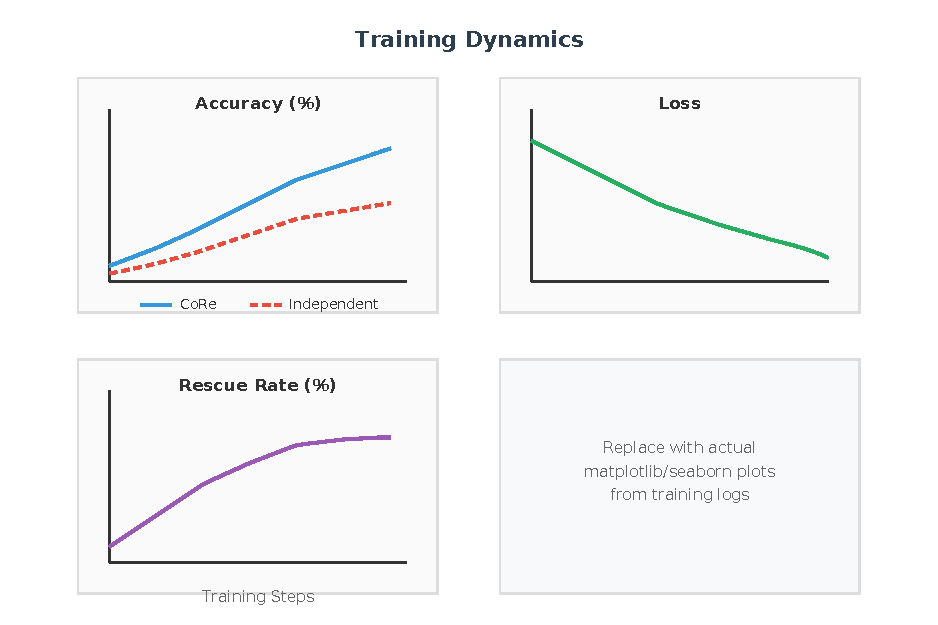
\includegraphics[width=\columnwidth]{figures/training_curves.pdf}
    \caption{Training curves showing accuracy, loss, and rescue rate over training steps. Rescue rate initially increases as models learn to use hints, then stabilizes.}
    \label{fig:training_curves}
\end{figure}

Figure~\ref{fig:training_curves} shows training dynamics. Notable observations:
\begin{itemize}
    \item Accuracy improves steadily, with collaborative training consistently outpacing independent training.
    \item Rescue rate increases during early training as models learn to leverage hints, then plateaus around 20\%.
    \item Loss becomes negative (for GRPO/SAPO), indicating successful policy improvement relative to the reference.
\end{itemize}

\section{Discussion}

\paragraph{Why does collaboration help?}
Our analysis suggests two mechanisms: (1) \textbf{Complementary coverage}---different models solve different subsets of problems, and collaboration enables access to peer solutions. (2) \textbf{Knowledge transfer}---through the rescue mechanism, models learn problem-solving strategies from peers without explicit distillation.

\paragraph{Limitations.}
Our framework requires training multiple models simultaneously, increasing computational cost. The rescue mechanism depends on hint quality, which may degrade for very complex problems. Future work could explore more sophisticated hint construction or multi-round collaboration.

\paragraph{Broader Impact.}
\methodname{} demonstrates that LLMs can benefit from collaborative training, analogous to human collaborative learning. This opens avenues for training specialized model ``teams'' for complex reasoning tasks.

\section{Conclusion}

We introduced \fullmethodname{} (\methodname{}), a framework for training multiple LLMs to reason collaboratively through cross-model teaching. Our rescue mechanism enables models to learn from peer successes, recovering 15-25\% of initially-failed problems. Experiments on GSM8K and MATH demonstrate consistent improvements over independent training and ensemble baselines. We hope this work inspires further research into collaborative multi-model learning for complex reasoning.

\section*{Limitations}

Our work has several limitations:
\begin{itemize}
    \item \textbf{Computational cost}: Training multiple models simultaneously requires more resources than single-model training.
    \item \textbf{Model pairing}: We explored only pairwise collaboration; larger groups may have different dynamics.
    \item \textbf{Domain specificity}: Our experiments focus on mathematical reasoning; generalization to other domains requires validation.
    \item \textbf{Hint construction}: Our extractive summarization for hints may lose nuanced reasoning; learned compression could improve.
\end{itemize}

\section*{Ethics Statement}

This work focuses on improving mathematical reasoning capabilities in LLMs. We do not anticipate negative societal impacts from the methods themselves. All experiments use publicly available models and datasets.

\bibliography{references}

\appendix

\section{Implementation Details}
\label{sec:appendix_implementation}

\subsection{LoRA Configuration}
We apply LoRA to the following modules: \texttt{q\_proj}, \texttt{k\_proj}, \texttt{v\_proj}, \texttt{o\_proj}, \texttt{gate\_proj}, \texttt{up\_proj}, \texttt{down\_proj}. This results in approximately 30M trainable parameters per 3B model (~0.96\% of total).

\subsection{Hint Construction Details}
Hints are constructed by:
\begin{enumerate}
    \item Extracting the successful solution trace
    \item Identifying key reasoning steps using sentence embeddings
    \item Truncating to $L_{\max}$ tokens while preserving sentence boundaries
    \item Formatting with special tokens: \texttt{<hint>}...\texttt{</hint>}
\end{enumerate}

\subsection{Reward Weights}
Default reward weights: $w_1 = 1.0$ (exploit), $w_2 = 0.2$ (explore), $w_3 = 0.3$ (cross-model).

\section{Additional Results}
\label{sec:appendix_results}

\subsection{Per-Category MATH Results}

\begin{table}[h]
    \centering
    \small
    \begin{tabular}{lcc}
        \toprule
        \textbf{Category} & \textbf{Independent} & \textbf{\methodname{}} \\
        \midrule
        Algebra & 42.1 & 48.3 \\
        Counting & 24.5 & 31.2 \\
        Geometry & 18.3 & 25.7 \\
        Number Theory & 31.8 & 38.4 \\
        Prealgebra & 58.2 & 63.1 \\
        Precalculus & 22.4 & 29.8 \\
        Intermediate Algebra & 15.6 & 22.3 \\
        \bottomrule
    \end{tabular}
    \caption{Per-category results on MATH.}
    \label{tab:math_categories}
\end{table}

\subsection{Training Efficiency}

\begin{table}[h]
    \centering
    \small
    \begin{tabular}{lcc}
        \toprule
        \textbf{Method} & \textbf{GPU Hours} & \textbf{Acc/Hour} \\
        \midrule
        Independent ($\times 2$) & 48 & 1.30 \\
        \methodname{} & 72 & 1.00 \\
        \bottomrule
    \end{tabular}
    \caption{Training efficiency comparison.}
    \label{tab:efficiency}
\end{table}

\end{document}
